\documentclass[aspectratio=169]{beamer}

\usepackage{tikz}
\usetikzlibrary{shadows}
\usepackage{listings}
\usepackage[utf8,latin1]{inputenc}
\usepackage[natbibapa]{apacite}
\usepackage{multirow}
\usepackage{color, colortbl}
\usepackage{tcolorbox}

\makeatletter \def\newblock{\beamer@newblock} \makeatother

\beamertemplatenavigationsymbolsempty
\setbeamertemplate{itemize items}[circle]
\setbeamertemplate{section in toc}[circle]
\mode<beamer>{\setbeamercolor{math text displayed}{fg=iwmgray}}
\setbeamercolor{block body}{bg=iwmorange!50!white}
\setbeamercolor{block title}{fg=white, bg=iwmorange}

\definecolor{iwmorange}{RGB}{255,105,0}
\definecolor{iwmgray}{RGB}{67,79,79}
\definecolor{iwmblue}{RGB}{60,180,220}
\definecolor{iwmgreen}{RGB}{145,200,110}
\definecolor{iwmpurple}{RGB}{120,0,75}

\setbeamercolor{title}{fg=iwmpurple}
\setbeamercolor{frametitle}{fg=iwmpurple}
\setbeamercolor{structure}{fg=iwmpurple}
\setbeamercolor{normal text}{fg=iwmgray}
\setbeamercolor{author}{fg=iwmgray}
\setbeamercolor{date}{fg=iwmgray}

\lstset{language = R,%
  basicstyle = \ttfamily\color{iwmgray},
  %frame = single,
  rulecolor = \color{iwmgray},
  commentstyle = \slshape\color{iwmgreen},
  keywordstyle = \bfseries\color{iwmgray},
  identifierstyle = \color{iwmpurple},
  stringstyle = \color{iwmblue},
  numbers = none,%left,numberstyle = \tiny,
  basewidth = {.5em, .4em},
  showstringspaces = false,
  emphstyle = \color{red!50!white}}

\setbeamercolor{graybox}{bg=iwmgray!30}
\newenvironment{colbox}[1][\textwidth]%
  {\begin{beamercolorbox}[wd=#1, rounded=true, shadow=true]{graybox}}
  {\end{beamercolorbox}}

\AtBeginSection[]{
  \frame{
    \tableofcontents[sectionstyle=show/hide, subsectionstyle=show/show/hide]}}

% \setbeamertemplate{headline}{
%  \begin{beamercolorbox}{section in head}
%    \vskip5pt\insertsectionnavigationhorizontal{\paperwidth}{}{}\vskip2pt
%  \end{beamercolorbox}
% }

\setbeamertemplate{footline}{\vskip-2pt\hfill\insertframenumber$\;$\vskip2pt}

\title{Simulation-based power analysis}
\author{Nora Wickelmaier}
%\institute{Leibniz-Institut f\"ur Wissensmedien, T\"ubingen}
\date{Last modified: 2025-09-11}


\begin{document}

\begin{frame}
\thispagestyle{empty}
\titlepage
\end{frame}

\begin{frame}{}%{Can effect sizes be too large?}
  %\pause
  \begin{center}\huge{Help, my effect size is too large!}\end{center}
    \vspace{.2cm}
  \pause
  \begin{itemize}
    \item Probably never heard anyone complain about this
    \item But it is a huge problem for the scientific integrity of our field
    \item Reported effect sizes in the literature are way too large\\[4ex]
      \pause
    \item We will look at an example from the literature: \\
     Decision biases from two-hand tapping
  \end{itemize}
  \vfill
\end{frame}


\begin{frame}{Refresher: Framing}

\begin{itemize}
\item \citet{ TverskyKahneman81}\\[1ex]

``Imagine that the U.S.\ is preparing for the outbreak of an unusual Asian
disease, which is expected to kill 600 people. Two alternative programs to
combat the disease have been proposed'' (p.~453)\\[1ex]

\begin{columns}
\begin{column}{0.4 cm}
\end{column}
%
\begin{column}{5.8 cm}
\begin{colbox}
If Program A is adopted \textbf{200} people will be \textbf{saved} [109]\\[2ex]

If Program B is adopted there is 1/3 probability that \textbf{600} people
will be \textbf{saved}, and 2/3 probability that \textbf{no people} will be
\textbf{saved} [43]
\end{colbox}
\end{column}
%
\begin{column}{5.8 cm}
\begin{colbox}
If Program C is adopted \textbf{400} people will
\textbf{die} [34]\\[2ex]

If Program D is adopted there is 1/3 probability that \textbf{nobody} will
\textbf{die}, and 2/3 probability that\\
\textbf{600} people will \textbf{die} [121]
\end{colbox}
\end{column}
\end{columns}

\vspace{2ex}

\item Odds ratio (OR) $=$ 9.0
\end{itemize}
\end{frame}

\begin{frame}[fragile]{Decision biases from two-hand tapping}

\begin{itemize}
\item \citet{McElroySeta04}, $n = 48$\\[1ex]

``a behavioral task of finger tapping was used to induce asymmetrical
activation of the respective hemispheres \dots Framing effects were found when
the right hemisphere was selectively activated whereas they were not observed
when the left hemisphere was selectively activated'' (p.~572)

\begin{lstlisting}
     right-hand tapping  left-hand tapping  ratio of odds
     safe risky          safe risky         ratios (ROR)
gain    8     4            12     1
loss    7     4             3     9
OR          1.1                  36         31.5
\end{lstlisting}

\item Our replication \citep[see][]{Gelman20}, $n = 332$
\begin{lstlisting}
gain   52    31            56    27
loss   26    57            30    53
OR          3.7                 3.7          1.0
\end{lstlisting}
\end{itemize}

\end{frame}


\begin{frame}{Large effects from subtle manipulations?}

There is a simple explanation for the seemingly large effects published all
over the psychological literature\\[2ex]

\begin{itemize}
\item that works without any real large effects

\item but assumes that they are statistical artifacts based on a combination
of\\[2ex]

~\hfill\begin{colbox}[5cm]
\centering
low power\\
$\wedge$\\
selection by significance\\[1ex]
\hrule\vspace{1ex}
$\Rightarrow$ inflated effect
\end{colbox}\hfill~

\vspace{2ex}

\citep[type M error;][]{GelmanCarlin14}
\end{itemize}

\end{frame}

\begin{frame}{Classical inference in a nutshell}

\begin{itemize}
\item Deciding between two hypotheses about parameter of data-generating
model \citep{NeymanPearson33}

\item Null hypothesis (specific), alternative hypothesis (logical opposite)\\
-- Example: Binomial model, H$_0$: $\pi = 0.5$, H$_1$: $\pi \neq 0.5$

\item Possible decision errors\\[1ex]

\renewcommand{\arraystretch}{1.2}
\begin{columns}
\begin{column}{7cm}
\begin{colbox}[7.6cm]
\centering
\begin{tabular}{l|c|c|}
\multicolumn{1}{l}{} & \multicolumn{1}{c}{Decision for H$_0$}
 & \multicolumn{1}{c}{Decision for H$_1$}\\ \cline{2-3}
H$_0$ true & correct                & type I error, $\alpha$\\ \cline{2-3}
H$_1$ true & type II error, $\beta$ & correct               \\ \cline{2-3}
\end{tabular}
\end{colbox}
\end{column}
%
\begin{column}{3cm}
Conventions
\begin{itemize}
\item $\alpha = 0.05$
\item $\beta < 0.2$
\end{itemize}
\end{column}
\end{columns}

\vspace{1ex}

\item Decision based on data (p-value)\\
-- If $p < \alpha$, choose H$_1$; else retain H$_0$

\item Power $= 1 - \beta$\\
-- Probability of test to detect an effect of a given size
\end{itemize}

\end{frame}

\begin{frame}{Power function}

\begin{columns}
\begin{column}{4.5cm}
Power of a test depends on\\[1ex]

\begin{itemize}
\item effect size\\
(deviation from H$_0$)

\item sample size $n$

\item $\alpha$\\[2ex]
\end{itemize}

With effect size, power, and $\alpha$ fixed, we can calculate $n$
\end{column}
%
\begin{column}{10cm}
\includegraphics[width=10cm]{../figures/OCbinomtest}
\end{column}
\end{columns}

\end{frame}

\begin{frame}{High power is a necessary condition for valid inference}

\begin{columns}
\begin{column}{7.9cm}
\includegraphics[width=7.9cm]{../figures/birthdiff10}
\end{column}
%
\begin{column}{7.9cm}
\includegraphics[width=7.9cm]{../figures/birthdiff80}
\end{column}
\end{columns}

\vspace{2ex}

``If power is low \dots every possible outcome under repeated sampling will
be misleading: there will be a high proportion of inconclusive null results,
and any significant effects will be due to mis-estimations of the true
effect'' \citep[][p.~1317]{VasishthGelman21}

\end{frame}

\begin{frame}{Power analysis by simulation}

Why simulation?\\[1ex]
\begin{itemize}
\item Simulation is at the heart of statistical inference

\item Inference: Compare the data with the output of a statistical model

\item If data look different from model output, reject model (or its
assumptions)

\item Simulation forces us to {\bf specify a data model} and to attach
  meaning to its components

\item Model should not be totally unrealistic for those aspects of the world
we want to learn about
\end{itemize}

\end{frame}

% How does one assure that the power of an experiment is high enough? And,
% first of all, how does one calculate the power of a planned test? This guide
% addresses both questions by computer simulation. But why calculate power by
% self-made simulation rather than by readily available software? Simulation
% forces us to specify a data model and to attach meaning to its components.
% This in turn will facilitate drawing valid inferences from the statistical
% test. After all, it is the model and its implications that the test
% confronts with empirical observations. Understanding what exactly is
% rejected if the test becomes significant, will improve our conclusions.


\begin{frame}{Power simulation}

%The steps in general\\[1ex]

\begin{colbox}
\begin{enumerate}
\item Specify the model including the effect of interest

\item Generate observations from the model

\item Test H$_0$

\item Repeat
\end{enumerate}
\end{colbox}

\vspace{3ex}

%Power is estimated from the proportion of significant test results
Power corresponds to how often a test obtains a significant result for a given $\alpha$ level (e.g.~5\%), given that an effect is truly present
\vspace{0.4cm}
\begin{equation*}
\widehat{Power}_s = \frac{\sum_{i = 1}^{niter} I(\mbox{\emph{p-value}}_{is} < \alpha | H_1)}{niter}
\end{equation*}


\end{frame}

% Ad 2: Once the data-generating model is fully specified, it can be used to
% draw observations from it. In R, functions like \verb+rbinom()+ or
% \verb+rnorm()+ will accomplish this. The number of draws equals the planned
% sample size of the experiment. Care has to be taken that the random sampling
% from the model reflects the design of the study. If there are dependencies
% in the data, as there are with repeated measures, the model has to produce
% correlated observations (for an example, see \ref{sec:pairtwosamplet}).
% These correlations have to be pre-specified as well.
%
% Ad 3: With the model-generated observations at hand one performs a test of
% H$_0$. The test should be the same as that which will be used to analyze the
% actual data, or else the power of the interesting test will remain unknown.


\begin{frame}{Specify the model including the effect of interest}

(1) Choose statistical model according to its assumptions
\begin{itemize}
\item Binomial test $\to$ binomial distribution $\to$ \texttt{rbinom()}

\item t test $\to$ normal distribution $\to$ \texttt{rnorm()}

\item \dots\\[1ex]
\end{itemize}

(2) Fix unknown quantities
\begin{itemize}
\item Standard deviations, correlations, \dots \\[1ex]
%\item Plausible values from the literature (beware of significance filter)
\end{itemize}

(3) Specify the effect of interest
\begin{itemize}

%\item \emph{Not} the true effect (else no need to run the study!)

\item \emph{Not} the effect one expects or hopes to find (size of effect is
unknown!)

\item \emph{Never} an effect size taken from another study (significance
filter!)

\item \emph{But} the biologically or clinically or psychologically ``relevant
effect one would regret missing'' \citep{Harrell20}
\end{itemize}

\end{frame}

\begin{frame}[fragile]{Estimating power with simulation}
  {Pseudo Code}

\begin{lstlisting}
  Set sample size to n
  replicate
  {
    Draw sample from model with minimum relevant effect
    Test null hypothesis
  }
  Determine proportion of significant results
\end{lstlisting}

\vspace{2ex}

Sample size calculation\\[1ex]

\begin{itemize}
\item Sample size $n$, minimal relevant effect and $\alpha$ must be
predetermined

\item Adjust $n$ until desired power ($0.8$ or $0.95$) is reached

\item To be on the safe side, assume higher variation, less (or more)
correlation, and smaller interesting effects (what results can we expect, if
\dots)
\end{itemize}

\end{frame}

\begin{frame}{Example: How to fix the two-hand tapping study?}
  {1. Specify model}
  \begin{itemize}
    \item Logit model with interaction
  \[
  \log \frac{p}{1 - p} = \beta_0
                  + \beta_1 \cdot \text{left hand}
                  + \beta_2 \cdot \text{gain}
                  + \beta_3 \cdot (\text{left hand} \times \text{gain})
\]
    \item Suggest a minimum relevant effect
      \begin{itemize}
        \item We can look at the original framing effect study and its many replications
        \item Former study by \citet{McElroySeta03} found $ROR = 3.4$ for
          similar manipulation
        \item Other studies investigating influencing factors
        \citep[with RORs $\approx$ 2--3, e.\,g., foreign language
      effect,][]{CostaFoucart14, Wickelmaier15}
        %\item Other theoretical assumptions?
      \end{itemize}
    \item Underlying distribution: $X \sim Binom(n, p)$
  \end{itemize}
\end{frame}

% Some background
% 
% Original framing effect \citep{TverskyKahneman81}
% - Odds for safe choice: about 2:1 in gain frame vs.\ 1:2 in loss frame
% - OR approx 4
% 
% Manipulation of framing effect
% - Foreign-language effect \citep{CostaFoucart14, Wickelmaier15}:
%   ROR approx 2-3
% 
% Suggesting a minimum relevant effect
% 
% With right-hand tapping, framing effect is halved
% - OR $=$ 2, $\sqrt{2}$:1 vs.\ 1:$\sqrt{2}$
% 
% With left-hand tapping, framing effect is doubled
% - OR $=$ 8, $\sqrt{8}$:1 vs.\ 1:$\sqrt{8}$
% 
% ROR = 4
% 
% log(1:sqrt(2))
% log(1/2)
% log(2)
% log(4)


\begin{frame}{Example: How to fix the two-hand tapping study?}
  {1. Specify model}
\begin{columns}
\begin{column}{8cm}
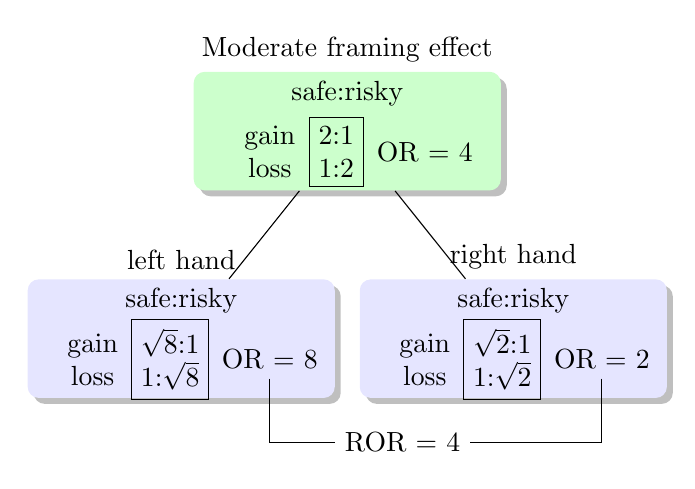
\begin{tikzpicture}
[x=40, y=25,
 every node/.style={align=center},
 nodeOut/.style={fill=blue!10, rounded corners, minimum width=3.9cm,
   drop shadow},
 nodeOR/.style={draw}
]
\node[nodeOut, fill=green!20,
  label={Moderate framing effect}] (O1) at ( 0,  4.3) {safe:risky\\[4ex]};
\node                at (-0.7, 4)  {gain\\ loss};
\node[nodeOR]        at (-0.1, 4) {2:1\\ 1:2};
\node                at ( 0.7, 4) {OR $=$ 4};
\node[nodeOut, label={left hand}] (O2) at (-1.5, 1.3) {safe:risky\\[4ex]};
\node                at (-2.3, 1)  {gain\\ loss};
\node[nodeOR]        at (-1.6, 1) {$\sqrt{8}$:1\\ 1:$\sqrt{8}$};
\node           (R8) at (-0.7, 1) {OR $=$ 8};
\node[nodeOut, label={right hand}] (O3) at ( 1.5, 1.3) {safe:risky\\[4ex]};
\node                at ( 0.7, 1)  {gain\\ loss};
\node[nodeOR]        at ( 1.4, 1) {$\sqrt{2}$:1\\ 1:$\sqrt{2}$};
\node           (R2) at ( 2.3, 1) {OR $=$ 2};
\node           (O4) at (0.5, -0.2) {ROR $=$ 4};
\draw (O1) -- (O2);
\draw (O1) -- (O3);
\draw (R8) -- (-0.7, -0.2) -- (O4);
\draw (R2) -- ( 2.3, -0.2) -- (O4);
\end{tikzpicture}
\end{column}
\begin{column}{6cm}
  Translating into parameters
  \begin{itemize}
    \item $\exp(\beta_0) = \frac{1}{\sqrt{2}}$\\
      odds in reference categories: right and loss
    \item $\exp(\beta_1) = \frac{1}{2}$\\
      OR of switching to left hand
    \item $\exp(\beta_2) = 2$\\
      OR of switching to gain frame
    \item $\exp(\beta_3) = 4$\\
      ROR
  \end{itemize}
\end{column}
\end{columns}
\vfill
\[
  \log \frac{p}{1 - p} = \beta_0
                  + \beta_1 \cdot \text{left hand}
                  + \beta_2 \cdot \text{gain}
                  + \beta_3 \cdot (\text{left hand} \times \text{gain})
\]

\end{frame}

\begin{frame}[fragile]{Example: How to fix the two-hand tapping study?}
  {2. Generate observations}
  \begin{itemize}
    \item Calculate logits for the model
\begin{lstlisting}
n <- 100
dat <- read.table(header = TRUE, text = "
  hand frame
     r  gain
     r  loss
     l  gain
     l  loss")                                          # ref. cat.
dat$hand <- factor(dat$hand, levels = c("r", "l"))          #   right
dat$frame <- factor(dat$frame, levels = c("loss", "gain"))  #   loss

expbeta <- c(1/sqrt(2), 1/2, 2, 4)  # ROR = 4, linear on logit scale
logit <- model.matrix(~ hand * frame, dat) %*% log(expbeta)
\end{lstlisting}
  \end{itemize}
\end{frame}


\begin{frame}[fragile]{Example: How to fix the two-hand tapping study?}
  {2. Generate observations}
  \begin{itemize}
    \item Simulate data from binomial distribution
\begin{lstlisting}
y <- rbinom(4, size = n/4, prob = plogis(logit))

## Sim 1             Sim 2             ...
## hand frame  y     hand frame  y
##    r  gain  16       r  gain  15
##    r  loss  7        r  loss  13
##    l  gain  21       l  gain  19
##    l  loss  9        l  loss  7

\end{lstlisting}
  \end{itemize}
\end{frame}


\begin{frame}[fragile]{Example: How to fix the two-hand tapping study?}
  {3. Test H$_0$}
  \begin{itemize}
    \item Fit null model to your generated observations -- H$_0$: $
      \beta_3 = 0$
\begin{lstlisting}
m1 <- glm(cbind(y, n/4 - y) ~ hand + frame, binomial, dat)
\end{lstlisting}
    \item Fit specified model to your generated observations -- H$_1$:
      $\beta_3 \neq 0$
\begin{lstlisting}
m2 <- glm(cbind(y, n/4 - y) ~ hand * frame, binomial, dat)
## ROR = 5.880952
\end{lstlisting}
    \item Do a likelihood ratio test to test interaction
\begin{lstlisting}
anova(m1, m2, test = "LRT")
## Analysis of Deviance Table
## 
## Model 1: cbind(y, n/4 - y) ~ hand + frame
## Model 2: cbind(y, n/4 - y) ~ hand * frame
##   Resid. Df Resid. Dev Df Deviance Pr(>Chi)  
## 1         1     4.3436                       
## 2         0     0.0000  1   4.3436  0.03715

\end{lstlisting}
  \end{itemize}
\end{frame}


\begin{frame}[fragile]{Example: How to fix the two-hand tapping study?}
  {4. Repeat}
  \begin{itemize}
    \item Do previous steps repeatedly
\begin{lstlisting}
## Power analysis ##
n <- 300

pval <- replicate(2000, {
  y <- rbinom(4, size = n/4, prob = plogis(logit))
  mm1 <- glm(cbind(y, n/4 - y) ~ hand + frame, binomial, dat)
  mm2 <- glm(cbind(y, n/4 - y) ~ hand * frame, binomial, dat)
  anova(mm1, mm2, test = "LRT")$"Pr(>Chi)"[2]
})

mean(pval < 0.05)
## 0.7945
\end{lstlisting}
  \end{itemize}
\end{frame}


\begin{frame}{Final thoughts}

~\hfill\begin{colbox}[10cm]
Statistical tests are no screening procedures\\[1ex]
-- Significance is not a substitute for relevance\\
-- Nonsignificance does not imply absence of effect
\end{colbox}\hfill~

\vspace{2ex}

\begin{itemize}
\item Often, data are rather uninformative and compatible with many models and
hypotheses\\[1ex]

\item At the same time, ``all models are wrong'' \citep{Box76}\\[1ex]

\item Making data-based decisions using statistical inference requires a
confirmatory setting where a-priori substantive knowledge goes into the power
analysis\\[1ex]

\item When relying on statistical tests outside such a setting, all we do is
descriptive statistics with p-values; this does more harm than good

\item You can find a collection of worked out examples for power simulations in
  R in \citet{Wickelmaier22}: \url{https://doi.org/10.48550/arXiv.2110.09836}

\end{itemize}

\end{frame}


\appendix
\begin{frame}[allowframebreaks]{References}
\renewcommand{\bibfont}{\small}
\bibliographystyle{apacite}
\bibliography{../lit}
\end{frame}


\section*{Extra slides}


\begin{frame}{P-value}

\begin{colbox}
The p-value is the probability of obtaining a test statistic that signals a
deviation from H$_0$ at least as extreme as that observed in the experiment,
given H$_0$ is true and its underlying model holds
\end{colbox}

\vspace{2ex}
\url{http://apps.mathpsy.uni-tuebingen.de/fw/pvalbinom/}

\end{frame}


\begin{frame}{On the role of power}

\begin{itemize}
\item \citet{VasishthGelman21}\\[1ex]

``the importance of power cannot be stressed enough. Power should be seen as
the ball in a ball game; it is only a very small part of the sport, because
there are many other important components. But the players would look pretty
foolish if they arrive to play on the playing field without the ball. Of
course, power is not the only thing to consider in an experiment; no amount of
power will help if the design is confounded or introduces a bias in some
way'' (p.~1333)
\end{itemize}

\end{frame}

\end{document}

